
% https://pdfs.semanticscholar.org/1417/c585009393cc2b45a38939a5e818738c62ea.pdf

\section{Graph algorithms}

In this part, we will sum up the results for the graph algorithms. These are generally more complex and the existence of massively parallel and optimal algorithms is not always considered as possible. Indeed, they often require a great deal of dependence on results obtained at previous stages. And they mostly have task-parallelism, which is not the most suitable for graphics cards.

\subsection{List ranking}

The list ranking problem consists to:
Given a list of $N$ elements, each one identified by a unique address (identifier) and pointing to its successor. Let define the rank as the number of items between the head of the list and the item. The problem resides in finding the ranks of all the elements in the list.

The first parallel algorithm was proposed by J. C. Wyllie~\cite{wyllie1979complexity}, it simply consists in a path-doubling strategy, hence it was $O(\log N)$. But, this would lead to a work complexity of $O(N \log N)$ instead of $O(N)$ for the sequential version. R. J. Anderson and G. L. Miller proposes an enhancement by splicing out some elements from the list. This helps to subdivide the list into sublists on which they will apply the Wyllie algorithm. Then, they will need to reconstruct the general order based on the split elements~\cite{anderson1990simple}.

But, the complexity of list ranking is in $\Theta(\frac{N}{PB} \log_{\frac{M}{B}} \frac{N}{B})$ in PEM model of computation and is thus as complex as sorting a collection due to the distributed nature of the caches\index{Cache} and the difficulty to transfer information and its tight link with the permutation problem~\cite{jacob2014complexity}.

The main idea consists to create independent sets via 3-coloring ($\frac{N}{3}$ size), through the forward/backward edges algorithm or deterministic coin tossing ($\frac{N}{4}$ size), solve the subproblems and recompose the solution~\cite{chiang1995external}. This operation of decomposition and reconstruction of the list is called brigde-out/in, it consists in making a copy of the original list, sort the original by successor identifier, scanning through original and the copy together to obtain successor information and sort back the modified original list by identifier~\cite{jacob2014complexity}.

3-coloring can be done as followed, we color alternatively forward pointers in red and blue, and backwards, in green and blue; each node will have one color at the exception of head/tail who have two, it remains to color them as the head of the list. In practice, we need to put the nodes in a priority queue based on the index, because we can't access any element in any order, this would result in too many transfers, and a priority queue can have a complexity of $O(\frac{1}{B}\log_{\frac{M}{B}} \frac{N}{B}$)~\cite{arge2007optimal}.

Behind this curious problem, there is a fundamental operation which has many applications: broadcasting an information.

\begin{figure}[!htb]
    \centering
    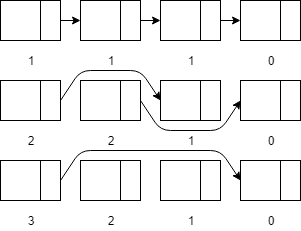
\includegraphics[width=0.5\linewidth]{Chapters/GPU/Algorithms/ListRanking.png} 
    \caption{List ranking}
\end{figure}

\subsection{Euler tour}

R. Tarjan and U. Vishkin introduced the Euler tour technique~\cite{tarjan1985efficient}; the Euler tour is defined as being able from one vertex of the graph to visit every edges exactly twice, in both direction. Hence, it can be easily mapped to a list ranking problem and this technique was used to solve many theoretical problems leading to several and various results to trees.

The bottom idea is that we can use the prefix sum algorithm through the Euler tour technique. This allows us to represent our tree structure as a flat collections of elements and apply our more advanced operations on all the elements without worrying on the accesses.

\subsection{Tree contraction}

Tree contraction was introduced by G .L. Miller and J. H. Reif in 1989~\cite{miller1989parallel} and has been used to design many and efficient parallel algorithms due to the possibility to represent the problems as a tree. The algorithm requires two primary operations:

\begin{itemize}
    \item Rake which removes all the leafs of a tree (merging childless nodes together).
    \item Compress consists to identify every vertex $v_{i}$ with $v_{i+1}$ when $i$ is odd and $v_{i}$ has only one child which is not leaf.
\end{itemize}

Both operations are successively repeated until the tree is reduced to one and unique node. The maximal number of iterations needed is bounded by $O(\log N)$. This helps us to work with any tree and guarantee $O(\log N)$ operations even with degenerated cases like linked list.

Many algorithms are based on this algorithm, the \textit{Arithmetic Expression Evaluation}, the \textit{Tree isomorphism} or to find the \textit{3-connected components} of a graph~\cite{miller1991parallel}. Those present a complexity in $O(\text{sort}_{P}(N))$ with $P \leq \frac{N}{B^{2} \log B}$.

\subsection{Lowest common ancestors}

The lowest common ancestor (LCA) of two nodes $v$ and $w$ in a tree $T$ is the lowest (i.e. deepest) node that has both $v$ and $w$ as descendants.

D. Harel and R. E. Tarjan showed that LCA queries can be answered in constant time after only linear preprocessing of the tree through \textit{Heavy path decomposition}~\cite{harel1984fast} but that data structure may be hard to implement. Arge et al., proposed to consider a simple $(\frac{M}{B})$-ary search tree\index{B-tree} which guarantees $O(\log_{\frac{M}{B}} \frac{N}{B})$ levels. The $K$ queries are treated after sorting the items, so that all of the queries can be answered by scanning the search tree a constant number of times through reduction of the problem to range minimum query (RMQ). The complexity is thus expressed as $O((1 + \frac{K}{N}) \text{sort}_{p}(N))$ I/Os.

\begin{figure}[!htb]
    \centering
    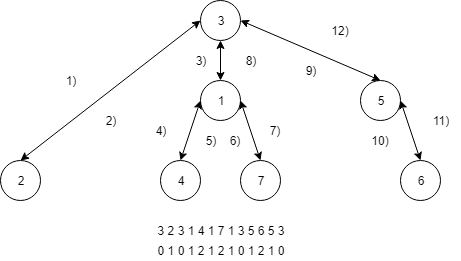
\includegraphics[width=0.8\linewidth]{Chapters/GPU/Algorithms/EulerTour.png} 
    \caption{LCA - RMQ: Euler tour}
\end{figure}

% Sparse table
% node prefix and suffix minima => http://wwwmayr.in.tum.de/lehre/2013WS/pa/split/sec-Tree-Algorithms-handout.pdf
% http://madalgo.au.dk/fileadmin/madalgo/OA_PDF_s/C269.pdf

\subsection{Connected and biconnected components, ear decomposition and minimum spanning tree}

Arge et al.~\cite{arge2010parallel} propose also many theoretical results in links to these problems:

Finding a minimum spanning tree, the connected components, the biconnected components and performing the ear decompositon can all be solved on the undirected connected graphs $G = (V, E)$ can be solved in $O(\text{sort}_{p}(|V|) + \text{sort}_{p}(|E|) \log(\frac{|V|}{PB})$ I/Os in the PEM model using up to $P \leq \frac{|V |+|E|}{B^{2} \log^{2} B}$ processors.

If the graph is sparse and closed under contraction, the connected components, the minimum spanning tree (if G is connected), the biconnected components and ear decomposition (if G is biconnected) can be computed in $O(\text{sort}_{p}(|V|))$ I/Os with $P \leq \frac{|V |+|E|}{B^{2} \log^{2} B}$.

Those results are extension of the work of Chiang et al.~\cite{chiang1995external} in external memory model. They relied on many other algorithms which would be out of the scope. These algorithms are often based on the Minimum Spanning Forest problem, where we divide the graphs among the processors. They all define a priority queue based on the weights of the concerned nodes and apply a Prim-like algorithm~\cite{arge2000external}. N. Zeh proposes a work in which he gathers many results with demonstrations and detailed explanations for the sequential I/O algorithms~\cite{zeh2002efficient}.